%% =======================================================
%% Actividad 10: Explorando distribuciones discretas
%%
%% Compilar desde actividades/: ./compilar.sh act10
%% Las figuras de img/ se generan con: python act10.py
%% =======================================================

%% ---- CONFIGURACIÓN ------------------------

\documentclass[11pt,letterpaper]{article}

\usepackage[indice]{tecnm}
\usepackage[T1]{fontenc}
\usepackage{amsmath}
\usepackage{xcolor}
\usepackage[most]{tcolorbox} % Carga tcolorbox con soporte para listings y saltos de página
\tcbuselibrary{listings, skins, breakable}
\setlength{\emergencystretch}{3em} % Evita líneas desbordadas por palabras en \texttt

% Paleta de colores (estilo GitHub Light / VS Code)
\definecolor{codebg}{HTML}{F8F9FA}       % Fondo del código
\definecolor{codehead}{HTML}{E9ECEF}     % Fondo de la barra de título
\definecolor{codeborder}{HTML}{CED4DA}   % Borde de la tarjeta
\definecolor{codetitle}{HTML}{212529}    % Texto del título
\definecolor{codekw}{HTML}{0550AE}       % Palabras clave (import, def, for...)
\definecolor{codefunc}{HTML}{8250DF}     % Funciones y métodos (describe, groupby...)
\definecolor{codestr}{HTML}{0A3069}      % Strings
\definecolor{codecomm}{HTML}{6E7781}     % Comentarios
\definecolor{codenum}{HTML}{8C959F}      % Números de línea
\definecolor{codeid}{HTML}{24292F}       % Texto general

% Configuración base de listings
\lstdefinestyle{pythonestilo}{
  language=Python,
  basicstyle=\ttfamily\footnotesize\color{codeid},
  keywordstyle=\color{codekw}\bfseries,
  keywordstyle=[2]\color{codefunc}, % Estilo secundario para métodos de datos
  stringstyle=\color{teal!80!black},
  commentstyle=\color{codecomm}\itshape,
  morekeywords={as, True, False, None, with, yield, lambda},
  morekeywords=[2]{print, len, sum, max, DataFrame, Series, value_counts, reindex, mean, std, var, randint, normal, seed, cumsum, poisson, binom, pmf, norm, fit, kde, bincount, linspace, train_test_split, make_blobs, GaussianNB, chisquare, pdf, cdf, hist, bar, plot, axhline, axvline, fill_between, subplots, figure, concat, nunique, load_iris, diff, sort, unique},
  numbers=left,
  numberstyle=\tiny\ttfamily\color{codenum},
  stepnumber=1,
  numbersep=10pt,
  showstringspaces=false,
  morestring=[b]{"""},
  tabsize=4,
  breaklines=true,
  breakatwhitespace=true,
  columns=flexible,
  keepspaces=true,
  literate=
    {á}{{\'a}}1 {é}{{\'e}}1 {í}{{\'i}}1 {ó}{{\'o}}1 {ú}{{\'u}}1
    {Á}{{\'A}}1 {É}{{\'E}}1 {Í}{{\'I}}1 {Ó}{{\'O}}1 {Ú}{{\'U}}1
    {ñ}{{\~n}}1 {Ñ}{{\~N}}1 {¿}{{?`}}1 {¡}{{!`}}1 {°}{{$^\circ$}}1
}

% Definición del entorno personalizado \begin{codigo}{Título}{etiqueta}
% \newtcblisting[auto counter, number within=section]{codigo}[2][]{
\newtcblisting[auto counter]{codigo}[2][]{
  listing only,
  breakable,                    % Permite que el bloque se divida si pasa de página
  enhanced,
  colback=codebg,
  colframe=codeborder,
  colbacktitle=codehead,
  coltitle=codetitle,
  fonttitle=\bfseries\small\sffamily,
  boxrule=0.6pt,
  arc=4pt,                      % Bordes redondeados
  left=20pt,                    % Espacio izquierdo para los números de línea
  right=8pt,
  top=6pt,
  bottom=6pt,
  toptitle=4pt,
  bottomtitle=4pt,
  before skip=12pt,
  after skip=12pt,
  listing options={style=pythonestilo},
  title={Código \thetcbcounter: #2},
  #1
}

% Paleta para salida de consola (estilo terminal limpia)
\definecolor{termbg}{HTML}{212529}      % Fondo oscuro tipo terminal
\definecolor{termhead}{HTML}{343A40}    % Barra superior
\definecolor{termtext}{HTML}{F8F9FA}    % Texto claro de alta legibilidad
\definecolor{termborder}{HTML}{495057}  % Borde

% Entorno \begin{consola}[label=out:iris]{Título}
\newtcblisting[auto counter]{consola}[2][]{
  listing only,
  breakable,
  colback=termbg,
  colframe=termborder,
  colbacktitle=termhead,
  coltitle=termtext,
  colupper=termtext,
  fonttitle=\bfseries\small\sffamily,
  boxrule=0.6pt,
  arc=4pt,
  left=8pt,
  right=8pt,
  top=6pt,
  bottom=6pt,
  toptitle=4pt,
  bottomtitle=4pt,
  before skip=12pt,
  after skip=12pt,
  listing options={
    basicstyle=\ttfamily\scriptsize\color{termtext}, % \scriptsize evita que las tablas de Pandas se partan de línea
    breaklines=true,
    columns=fixed,        % Mantiene alineadas las columnas de Pandas
    keepspaces=true,
    showstringspaces=false,
    literate=
      {á}{{\'a}}1 {é}{{\'e}}1 {í}{{\'i}}1 {ó}{{\'o}}1 {ú}{{\'u}}1
      {Á}{{\'A}}1 {É}{{\'E}}1 {Í}{{\'I}}1 {Ó}{{\'O}}1 {Ú}{{\'U}}1
      {ñ}{{\~n}}1 {Ñ}{{\~N}}1 {°}{{$^\circ$}}1
  },
  title={Salida \thetcbcounter: #2},
  #1
}

%% ---- DATOS DE LA MATERIA ------------------------

\materia{Modelos Estadísticos para el Aprendizaje \\ Automático y Ciencia de Datos}
\actividad{Tema 2.2
Distribuciones de Probabilidad Discretas y Continuas \\ Actividad 10 - Explorando Distribuciones Discretas}

\profesor{Dr. José Ismael Ojeda Campaña}
%\fecha{15 de octubre de 2026}    % opcional; por defecto es la fecha de hoy

\begin{document}
\portada
\indicegeneral

%% ---- CONTENIDO ---------------------------------

\section{Introducción}

Una variable aleatoria discreta toma valores que se cuentan: el número de éxitos en una serie de ensayos, el número de llamadas en una hora o el número de intentos hasta ganar. Cada distribución discreta resume las probabilidades de uno de estos patrones de conteo y tiene parámetros que fijan su forma \parencite{tecnm2026_documento_fuente,brownlee2020}.

En este documento se estudian las cinco distribuciones discretas del tema: Bernoulli, binomial, Poisson, geométrica e hipergeométrica. Cada una se simula con 10\,000 valores y con dos conjuntos distintos de parámetros, se grafican las frecuencias simuladas junto con la función de masa teórica y se comparan los resultados con las fórmulas de manera numérica: medias, varianzas, probabilidades puntuales y una prueba chi-cuadrada de bondad de ajuste. También se reproduce el ejemplo de la lotería de California del documento fuente y se muestra cómo disminuye el error de la simulación al aumentar el número de valores simulados. Al final se discute en qué fenómenos se aplica cada distribución y cómo cambia su forma con los parámetros.

\section{Marco conceptual}

\subsection{Distribuciones discretas}

Una distribución de probabilidad discreta resume las probabilidades de una variable aleatoria discreta mediante su función de masa de probabilidad $P(X = k)$, cuyos valores suman 1 \parencite{tecnm2026_documento_fuente}. Las cinco distribuciones de esta actividad se resumen en la Tabla~\ref{tab:resumen}, con su función de masa, su media y su varianza \parencite{tecnm2026_documento_fuente,rice2006}.

\begin{table}[htbp]
\centering
\caption{Distribuciones discretas de la actividad.}
\label{tab:resumen}
\small
\renewcommand{\arraystretch}{1.6}
\begin{tabular}{llcc}
\hline
\textbf{Distribución} & \textbf{$P(X = k)$} & \textbf{Media} & \textbf{Varianza} \\
\hline
Bernoulli$(p)$ & $p^k(1-p)^{1-k}$, \; $k = 0, 1$ & $p$ & $p(1-p)$ \\
Binomial$(n, p)$ & $\binom{n}{k}p^k(1-p)^{n-k}$ & $np$ & $np(1-p)$ \\
Poisson$(\lambda)$ & $\dfrac{e^{-\lambda}\lambda^k}{k!}$ & $\lambda$ & $\lambda$ \\
Geométrica$(p)$ & $(1-p)^{k-1}p$, \; $k \ge 1$ & $1/p$ & $(1-p)/p^2$ \\
Hipergeométrica$(N, K, n)$ & $\dfrac{\binom{K}{k}\binom{N-K}{n-k}}{\binom{N}{n}}$ & $n\dfrac{K}{N}$ & $n\dfrac{K}{N}\left(1-\dfrac{K}{N}\right)\dfrac{N-n}{N-1}$ \\
\hline
\end{tabular}
\end{table}

\subsection{Bernoulli y binomial}

Una variable de Bernoulli solo toma los valores 1 (éxito) y 0 (fracaso), con probabilidades $p$ y $1 - p$. Es el bloque básico de las demás: la binomial cuenta los éxitos en $n$ ensayos de Bernoulli independientes con la misma probabilidad $p$, y por lo tanto es la suma de $n$ variables de Bernoulli \parencite{tecnm2026_documento_fuente}.

\subsection{Poisson}

La distribución de Poisson describe el número de veces que ocurre un evento en un intervalo fijo de tiempo o espacio, cuando los eventos son independientes y su tasa promedio $\lambda$ es constante. Es el límite de la binomial cuando $n \to \infty$ y $p \to 0$ con $np = \lambda$ \parencite{tecnm2026_documento_fuente}.

\subsection{Geométrica}

La distribución geométrica cuenta el número de ensayos de Bernoulli hasta, e incluyendo, el primer éxito: para que $X = k$ deben ocurrir $k - 1$ fracasos seguidos de un éxito. En el documento fuente se ejemplifica con el número de boletos de lotería que hay que comprar hasta el primero ganador, con $p = 1/9$ \parencite{tecnm2026_documento_fuente}.

\subsection{Hipergeométrica}

Si una urna con $N$ bolas contiene $K$ negras y se extraen $n$ bolas sin reemplazo, el número $X$ de bolas negras extraídas es hipergeométrico. A diferencia de la binomial, las extracciones no son independientes, porque cada una cambia la composición de la urna \parencite{tecnm2026_documento_fuente}.

\subsection{Comparación entre lo teórico y lo empírico}

La frecuencia relativa de un valor $k$ en $N$ simulaciones es una proporción, cuyo valor esperado es $P(X = k)$ y cuyo error estándar es $\sqrt{P(1 - P)/N}$. Por eso, las diferencias entre las frecuencias simuladas y las probabilidades teóricas son pequeñas y disminuyen aproximadamente como $1/\sqrt{N}$. Para evaluar el conjunto de la distribución se usa la prueba chi-cuadrada de bondad de ajuste, que compara las frecuencias observadas $O_i$ con las esperadas $E_i$ mediante $\chi^2 = \sum (O_i - E_i)^2/E_i$; su hipótesis nula es que los datos provienen de la distribución teórica \parencite{tecnm2026_documento_fuente,rice2006}.

\section{Descripción de la actividad}

\textbf{Objetivo:} Comprender el comportamiento de las principales distribuciones discretas (Bernoulli, binomial, Poisson, geométrica e hipergeométrica) mediante simulaciones computacionales, análisis gráfico y comparación de resultados teóricos y empíricos \parencite{tecnm2026_documento_fuente}.

La actividad consta de cuatro tareas:

\begin{description}
    \item[1) Simulación individual.] Implementar en Python al menos dos distribuciones discretas distintas, con valores diferentes de sus parámetros.
    \item[2) Visualización.] Generar gráficos de barras o histogramas para comparar la forma de las distribuciones simuladas.
    \item[3) Comparación teórica-empírica.] Calcular los valores teóricos de probabilidad con las fórmulas y compararlos con los resultados simulados.
    \item[4) Reflexión final.] Explicar en qué fenómenos del mundo real se aplica cada distribución y cómo influyen los parámetros en su forma.
\end{description}

\section{Desarrollo}

Las tareas se resolvieron en el script que utiliza \texttt{numpy}, \texttt{pandas}, \texttt{scipy} y \texttt{matplotlib}. Se implementaron las cinco distribuciones, cada una con dos conjuntos de parámetros, en lugar de las dos mínimas que pide la actividad. Las simulaciones usan la semilla 10 para que los resultados sean reproducibles, y las figuras se guardan como imágenes PNG en la carpeta \texttt{img/}. El Código~\ref{cod:comun} contiene las importaciones y la función auxiliar \texttt{guardar()}, que además muestra las figuras en pantalla cuando el código se ejecuta en un cuaderno. La tarea 4 es una reflexión y se desarrolla en la sección de resultados. El cuaderno interactivo puede consultarse en Google Colab:

\begin{center}
    \url{https://colab.research.google.com/drive/1egz1s02WVbF143TfA3ad5c6462J49HrY?usp=sharing}
\end{center}

\begin{codigo}[label=cod:comun]{Importaciones y función auxiliar}
import math
import os
import random

import matplotlib

# En Colab o Jupyter no existe __file__; ahí las figuras también se muestran en pantalla
EN_NOTEBOOK = '__file__' not in globals()
if not EN_NOTEBOOK:
    matplotlib.use('Agg')  # Como script, genera las figuras como archivos PNG sin abrir ventanas

import matplotlib.pyplot as plt
import numpy as np
import pandas as pd
from scipy import stats

pd.set_option('display.width', 110)

# Carpeta donde se guardan las figuras que se incluyen en el reporte
BASE = os.getcwd() if EN_NOTEBOOK else os.path.dirname(os.path.abspath(__file__))
CARPETA_IMG = os.path.join(BASE, 'img')
os.makedirs(CARPETA_IMG, exist_ok=True)


def guardar(nombre):
    """Guarda la figura actual en la carpeta img/ y la muestra si se ejecuta en un notebook."""
    plt.tight_layout()
    plt.savefig(os.path.join(CARPETA_IMG, nombre), dpi=150)
    if EN_NOTEBOOK:
        plt.show()
    plt.close()
\end{codigo}

\subsection{Tarea 1: Simulación individual}

Cada distribución se simuló con 10\,000 valores y dos conjuntos de parámetros, como se muestra en el diccionario \texttt{DISTRIBUCIONES} del Código~\ref{cod:t1}. La función \texttt{simular()} usa el generador de \texttt{numpy}. Además, siguiendo los ejemplos del documento fuente, se escribieron desde cero los simuladores de la Bernoulli, la geométrica (se repiten ensayos hasta el primer éxito) y la Poisson (método de Knuth, que multiplica números uniformes hasta que el producto baja de $e^{-\lambda}$), usando solo \texttt{random.random()}. Las funciones \texttt{pmf\_manual()} y \texttt{momentos\_teoricos()} contienen las fórmulas de la Tabla~\ref{tab:resumen}; \texttt{pmf\_scipy()} calcula lo mismo con \texttt{scipy.stats}.

\begin{codigo}[label=cod:t1]{Tarea 1: parámetros, simuladores y fórmulas}
# Cada distribución se simula con dos conjuntos distintos de parámetros.
N_SIM = 10000
SEMILLA = 10
COLORES = ['tab:blue', 'tab:orange']

# Parámetros (hipergeométrica: N = total de bolas, K = negras, n = extracciones)
DISTRIBUCIONES = {
    'Bernoulli':      [dict(p=0.3), dict(p=0.7)],
    'Binomial':       [dict(n=10, p=0.5), dict(n=20, p=0.2)],
    'Poisson':        [dict(lam=2), dict(lam=7)],
    'Geométrica':     [dict(p=0.5), dict(p=0.2)],
    'Hipergeométrica': [dict(N=50, K=10, n=10), dict(N=50, K=25, n=10)],
}


def etiqueta(par):
    """Texto con los parámetros, por ejemplo 'n = 10, p = 0.5'."""
    nombres = {'lam': '$\\lambda$'}
    return ', '.join(f'{nombres.get(k, k)} = {v:g}' for k, v in par.items())


def simular(dist, par, tam, rng):
    """Genera `tam` valores de la distribución con los parámetros `par`."""
    if dist == 'Bernoulli':
        return rng.binomial(1, par['p'], tam)
    if dist == 'Binomial':
        return rng.binomial(par['n'], par['p'], tam)
    if dist == 'Poisson':
        return rng.poisson(par['lam'], tam)
    if dist == 'Geométrica':
        return rng.geometric(par['p'], tam)  # número de pruebas hasta el primer éxito
    if dist == 'Hipergeométrica':
        return rng.hypergeometric(par['K'], par['N'] - par['K'], par['n'], tam)


def pmf_scipy(dist, par, k):
    """Función de masa de probabilidad calculada con scipy.stats."""
    if dist == 'Bernoulli':
        return stats.bernoulli.pmf(k, par['p'])
    if dist == 'Binomial':
        return stats.binom.pmf(k, par['n'], par['p'])
    if dist == 'Poisson':
        return stats.poisson.pmf(k, par['lam'])
    if dist == 'Geométrica':
        return stats.geom.pmf(k, par['p'])
    if dist == 'Hipergeométrica':
        return stats.hypergeom.pmf(k, par['N'], par['K'], par['n'])


def pmf_manual(dist, par, k):
    """Función de masa calculada a mano con las fórmulas del documento fuente (un valor k)."""
    if dist == 'Bernoulli':
        return par['p'] ** k * (1 - par['p']) ** (1 - k) if k in (0, 1) else 0.0
    if dist == 'Binomial':
        n, p = par['n'], par['p']
        return math.comb(n, k) * p ** k * (1 - p) ** (n - k) if 0 <= k <= n else 0.0
    if dist == 'Poisson':
        lam = par['lam']
        return math.exp(-lam) * lam ** k / math.factorial(k)
    if dist == 'Geométrica':
        return (1 - par['p']) ** (k - 1) * par['p'] if k >= 1 else 0.0
    if dist == 'Hipergeométrica':
        N, K, n = par['N'], par['K'], par['n']
        if k < max(0, n - (N - K)) or k > min(n, K):
            return 0.0
        return math.comb(K, k) * math.comb(N - K, n - k) / math.comb(N, n)


def momentos_teoricos(dist, par):
    """Media y varianza teóricas de cada distribución."""
    if dist == 'Bernoulli':
        p = par['p']
        return p, p * (1 - p)
    if dist == 'Binomial':
        n, p = par['n'], par['p']
        return n * p, n * p * (1 - p)
    if dist == 'Poisson':
        return par['lam'], par['lam']
    if dist == 'Geométrica':
        p = par['p']
        return 1 / p, (1 - p) / p ** 2
    if dist == 'Hipergeométrica':
        N, K, n = par['N'], par['K'], par['n']
        return n * K / N, n * (K / N) * (1 - K / N) * (N - n) / (N - 1)


rng = np.random.default_rng(SEMILLA)
muestras = {(d, i): simular(d, par, N_SIM, rng)
            for d, pares in DISTRIBUCIONES.items() for i, par in enumerate(pares)}

# Simulación "desde cero" con random.random(), como en el documento fuente
random.seed(SEMILLA)


def bernoulli_manual(p):
    return 1 if random.random() < p else 0


def geometrica_manual(p):
    pruebas = 1
    while random.random() >= p:
        pruebas += 1
    return pruebas


def poisson_manual(lam):
    # Método de Knuth: multiplicar uniformes hasta que el producto baje de e^(-lambda)
    L, k, prod = math.exp(-lam), 0, 1.0
    while prod > L:
        k += 1
        prod *= random.random()
    return k - 1


manuales = {
    'Bernoulli (p = 0.3)': [bernoulli_manual(0.3) for _ in range(N_SIM)],
    'Geométrica (p = 0.2)': [geometrica_manual(0.2) for _ in range(N_SIM)],
    'Poisson ($\\lambda$ = 7)': [poisson_manual(7) for _ in range(N_SIM)],
}
print(f"=== Tarea 1: simulación con {N_SIM} valores por caso (semilla {SEMILLA}) ===")
print("\nSimulación desde cero con random.random() (media muestral vs teórica):")
for nombre, valores in manuales.items():
    print(f"  {nombre.replace('$\\lambda$', 'lambda')}: media = {np.mean(valores):.3f}")
\end{codigo}

\subsection{Tarea 2: Visualización}

Para cada distribución se dibujaron, en una misma gráfica, las frecuencias relativas de las dos simulaciones como barras agrupadas, con la función de masa teórica como puntos negros (Figura~\ref{fig:comparacion}). La geométrica se recorta en $k = 20$ porque su cola es larga. En una segunda figura se variaron los parámetros de la binomial, la Poisson y la geométrica sobre las probabilidades teóricas (Figura~\ref{fig:parametros}).

\begin{codigo}[label=cod:t2]{Tarea 2: gráficos de barras y efecto de los parámetros}
fig, axes = plt.subplots(2, 3, figsize=(15, 8))
for ax, (dist, pares) in zip(axes.flat, DISTRIBUCIONES.items()):
    k_max = max(muestras[(dist, i)].max() for i in range(len(pares)))
    if dist == 'Geométrica':
        k_max = min(k_max, 20)  # la cola es larga; se muestran los primeros valores
    ks = np.arange(0, k_max + 1)
    ancho = 0.4
    for i, (par, color) in enumerate(zip(pares, COLORES)):
        frec = np.bincount(muestras[(dist, i)], minlength=k_max + 1)[:k_max + 1] / N_SIM
        ax.bar(ks + (i - 0.5) * ancho, frec, ancho, color=color, alpha=0.7,
               edgecolor='black', linewidth=0.4, label=f'Simulación: {etiqueta(par)}')
        ax.plot(ks + (i - 0.5) * ancho, pmf_scipy(dist, par, ks), 'k.', markersize=5)
    if dist == 'Bernoulli':
        ax.set_xticks([0, 1])  # solo toma los valores 0 y 1
    ax.set_title(dist)
    ax.set_xlabel('k')
    ax.set_ylabel('Frecuencia relativa')
    ax.legend(fontsize=7)
    ax.grid(axis='y', linestyle='--', alpha=0.5)
axes.flat[-1].axis('off')
axes.flat[-1].text(0.05, 0.5, 'Barras: frecuencias simuladas\nPuntos negros: P(X = k) teórica',
                   fontsize=11, va='center')
guardar('t2_comparacion_distribuciones.png')

# Cómo cambia la forma al variar un solo parámetro (probabilidades teóricas)
fig, axes = plt.subplots(1, 3, figsize=(15, 4.2))
k = np.arange(0, 31)
for p in [0.1, 0.5, 0.9]:
    axes[0].plot(k, stats.binom.pmf(k, 30, p), 'o-', markersize=3, label=f'n = 30, p = {p}')
axes[0].set_title('Binomial: efecto de p')
for lam in [1, 5, 15]:
    axes[1].plot(k, stats.poisson.pmf(k, lam), 'o-', markersize=3, label=f'$\\lambda$ = {lam}')
axes[1].set_title('Poisson: efecto de $\\lambda$')
for p in [0.2, 0.5, 0.8]:
    axes[2].plot(k[1:], stats.geom.pmf(k[1:], p), 'o-', markersize=3, label=f'p = {p}')
axes[2].set_title('Geométrica: efecto de p')
for ax in axes:
    ax.set_xlabel('k')
    ax.set_ylabel('P(X = k)')
    ax.legend(fontsize=8)
    ax.grid(linestyle='--', alpha=0.5)
guardar('t2_efecto_parametros.png')
\end{codigo}

\subsection{Tarea 3: Comparación teórica-empírica}

La comparación se hizo en cinco pasos: (a) medias y varianzas teóricas contra las simuladas; (b) probabilidades puntuales calculadas con la fórmula y comparadas con la frecuencia simulada y con el error estándar de una proporción (la fórmula manual se verifica contra \texttt{scipy} con \texttt{assert}); (c) prueba chi-cuadrada de bondad de ajuste, agrupando las categorías con frecuencia esperada menor que 5; (d) el ejemplo de la lotería de California del documento fuente, con 200\,000 sorteos simulados; y (e) el error máximo entre frecuencia y probabilidad para tamaños de simulación de 100 a 300\,000.

\begin{codigo}[label=cod:t3a]{Tarea 3a: media y varianza}
# a) Media y varianza
filas = []
for (dist, i), muestra in muestras.items():
    par = DISTRIBUCIONES[dist][i]
    media_t, var_t = momentos_teoricos(dist, par)
    filas.append({'Distribución': dist, 'Parámetros': etiqueta(par).replace('$\\lambda$', 'lambda'),
                  'Media teórica': media_t, 'Media simulada': muestra.mean(),
                  'Var. teórica': var_t, 'Var. simulada': muestra.var(ddof=1)})
tabla_momentos = pd.DataFrame(filas)
print("\n=== Tarea 3a: media y varianza, teóricas vs simuladas ===")
print(tabla_momentos.round(3).to_string(index=False))
\end{codigo}
\begin{codigo}[label=cod:t3b]{Tarea 3b: probabilidades puntuales}
# b) Probabilidades puntuales: fórmula manual, scipy y simulación
casos = [('Bernoulli', 0, 1), ('Binomial', 0, 5), ('Binomial', 1, 4), ('Poisson', 0, 2),
         ('Poisson', 1, 7), ('Geométrica', 0, 2), ('Geométrica', 1, 5),
         ('Hipergeométrica', 0, 1), ('Hipergeométrica', 1, 5)]
filas = []
for dist, i, kk in casos:
    par = DISTRIBUCIONES[dist][i]
    manual = pmf_manual(dist, par, kk)
    assert abs(manual - pmf_scipy(dist, par, kk)) < 1e-12  # la fórmula coincide con scipy
    empirica = np.mean(muestras[(dist, i)] == kk)
    # Error estándar de una proporción: raíz de p(1 - p) / N
    ee = math.sqrt(manual * (1 - manual) / N_SIM)
    filas.append({'Distribución': dist, 'Parámetros': etiqueta(par).replace('$\\lambda$', 'lambda'),
                  'k': kk, 'P teórica': manual, 'Frec. simulada': empirica,
                  'Diferencia': empirica - manual, 'Error estándar': ee})
tabla_puntual = pd.DataFrame(filas)
print("\n=== Tarea 3b: P(X = k) con la fórmula, y frecuencia simulada ===")
print(tabla_puntual.round(4).to_string(index=False))
\end{codigo}
\begin{codigo}[label=cod:t3c]{Tarea 3c: prueba chi-cuadrada de bondad de ajuste}
# c) Prueba chi-cuadrada de bondad de ajuste para cada simulación
filas = []
for (dist, i), muestra in muestras.items():
    par = DISTRIBUCIONES[dist][i]
    ks = np.arange(0, muestra.max() + 1)
    obs = np.bincount(muestra, minlength=len(ks)).astype(float)
    esp = pmf_scipy(dist, par, ks) * N_SIM
    # Se agrupan las categorías con frecuencia esperada menor que 5 (regla usual)
    grupos_o, grupos_e, acum_o, acum_e = [], [], 0.0, 0.0
    for o, e in zip(obs, esp):
        acum_o += o
        acum_e += e
        if acum_e >= 5:
            grupos_o.append(acum_o)
            grupos_e.append(acum_e)
            acum_o = acum_e = 0.0
    grupos_o[-1] += acum_o
    grupos_e[-1] += acum_e
    grupos_e = np.array(grupos_e) * (sum(grupos_o) / sum(grupos_e))  # iguala los totales
    chi2 = ((np.array(grupos_o) - grupos_e) ** 2 / grupos_e).sum()
    filas.append({'Distribución': dist, 'Parámetros': etiqueta(par).replace('$\\lambda$', 'lambda'),
                  'Categorías': len(grupos_o), 'chi2': chi2,
                  'p-valor': stats.chi2.sf(chi2, len(grupos_o) - 1)})
tabla_chi = pd.DataFrame(filas)
print("\n=== Tarea 3c: prueba chi-cuadrada de bondad de ajuste ===")
print(tabla_chi.round(4).to_string(index=False))
\end{codigo}
\begin{codigo}[label=cod:t3d]{Tarea 3d: lotería de California}
# d) Ejemplo del documento fuente: lotería de California (6 de 53)
ks = np.arange(0, 7)
teorica_loteria = np.array([pmf_manual('Hipergeométrica', dict(N=53, K=6, n=6), k) for k in ks])
sim_loteria = rng.hypergeometric(6, 47, 6, 200000)
frec_loteria = np.bincount(sim_loteria, minlength=7) / len(sim_loteria)
print("\n=== Tarea 3d: lotería de California (hipergeométrica N = 53, K = 6, n = 6) ===")
print(pd.DataFrame({'k': ks, 'P teórica': teorica_loteria,
                    'Frec. (200000 sorteos)': frec_loteria}).to_string(
    index=False, float_format=lambda v: f'{v:.6f}'))
\end{codigo}
\begin{codigo}[label=cod:t3e]{Tarea 3e: convergencia de la simulación}
# e) Convergencia: el error máximo baja al aumentar el número de simulaciones
tamanos = [100, 300, 1000, 3000, 10000, 30000, 100000, 300000]
rng_conv = np.random.default_rng(SEMILLA)
errores = {}
for dist in ['Binomial', 'Poisson', 'Geométrica']:
    par = DISTRIBUCIONES[dist][0]
    errores[dist] = []
    for tam in tamanos:
        m = simular(dist, par, tam, rng_conv)
        ks = np.arange(0, m.max() + 1)
        errores[dist].append(np.abs(np.bincount(m, minlength=len(ks)) / tam
                                    - pmf_scipy(dist, par, ks)).max())
plt.figure(figsize=(8, 4.5))
for dist, e in errores.items():
    plt.loglog(tamanos, e, 'o-', label=f'{dist} ({etiqueta(DISTRIBUCIONES[dist][0])})')
plt.loglog(tamanos, 1 / np.sqrt(tamanos), 'k--', alpha=0.5, label='$1/\\sqrt{N}$ (referencia)')
plt.title('Convergencia de la simulación a la distribución teórica')
plt.xlabel('Número de simulaciones N')
plt.ylabel('Máx. |frecuencia - P(X = k)|')
plt.legend(fontsize=8)
plt.grid(which='both', linestyle='--', alpha=0.5)
guardar('t3_convergencia.png')
print("\n=== Tarea 3e: error máximo según el número de simulaciones ===")
print(pd.DataFrame(errores, index=tamanos).rename_axis('N').round(4).to_string())

print(f"\nFiguras guardadas en {os.path.basename(CARPETA_IMG)}/")
\end{codigo}

\newpage
\section{Resultados}

\subsection{Tareas 1 y 2: Simulación y visualización}

\begin{consola}[label=out:t1]{Ejecución de \texttt{act10.py}: simuladores desde cero}
=== Tarea 1: simulación con 10000 valores por caso (semilla 10) ===

Simulación desde cero con random.random() (media muestral vs teórica):
  Bernoulli (p = 0.3): media = 0.295
  Geométrica (p = 0.2): media = 4.974
  Poisson (lambda = 7): media = 7.016
\end{consola}

Las medias de los simuladores escritos desde cero (0.295, 4.974 y 7.016) son cercanas a las teóricas (0.3, 5 y 7), por lo que producen valores con la distribución correcta.

\begin{figure}[htbp]
\centering
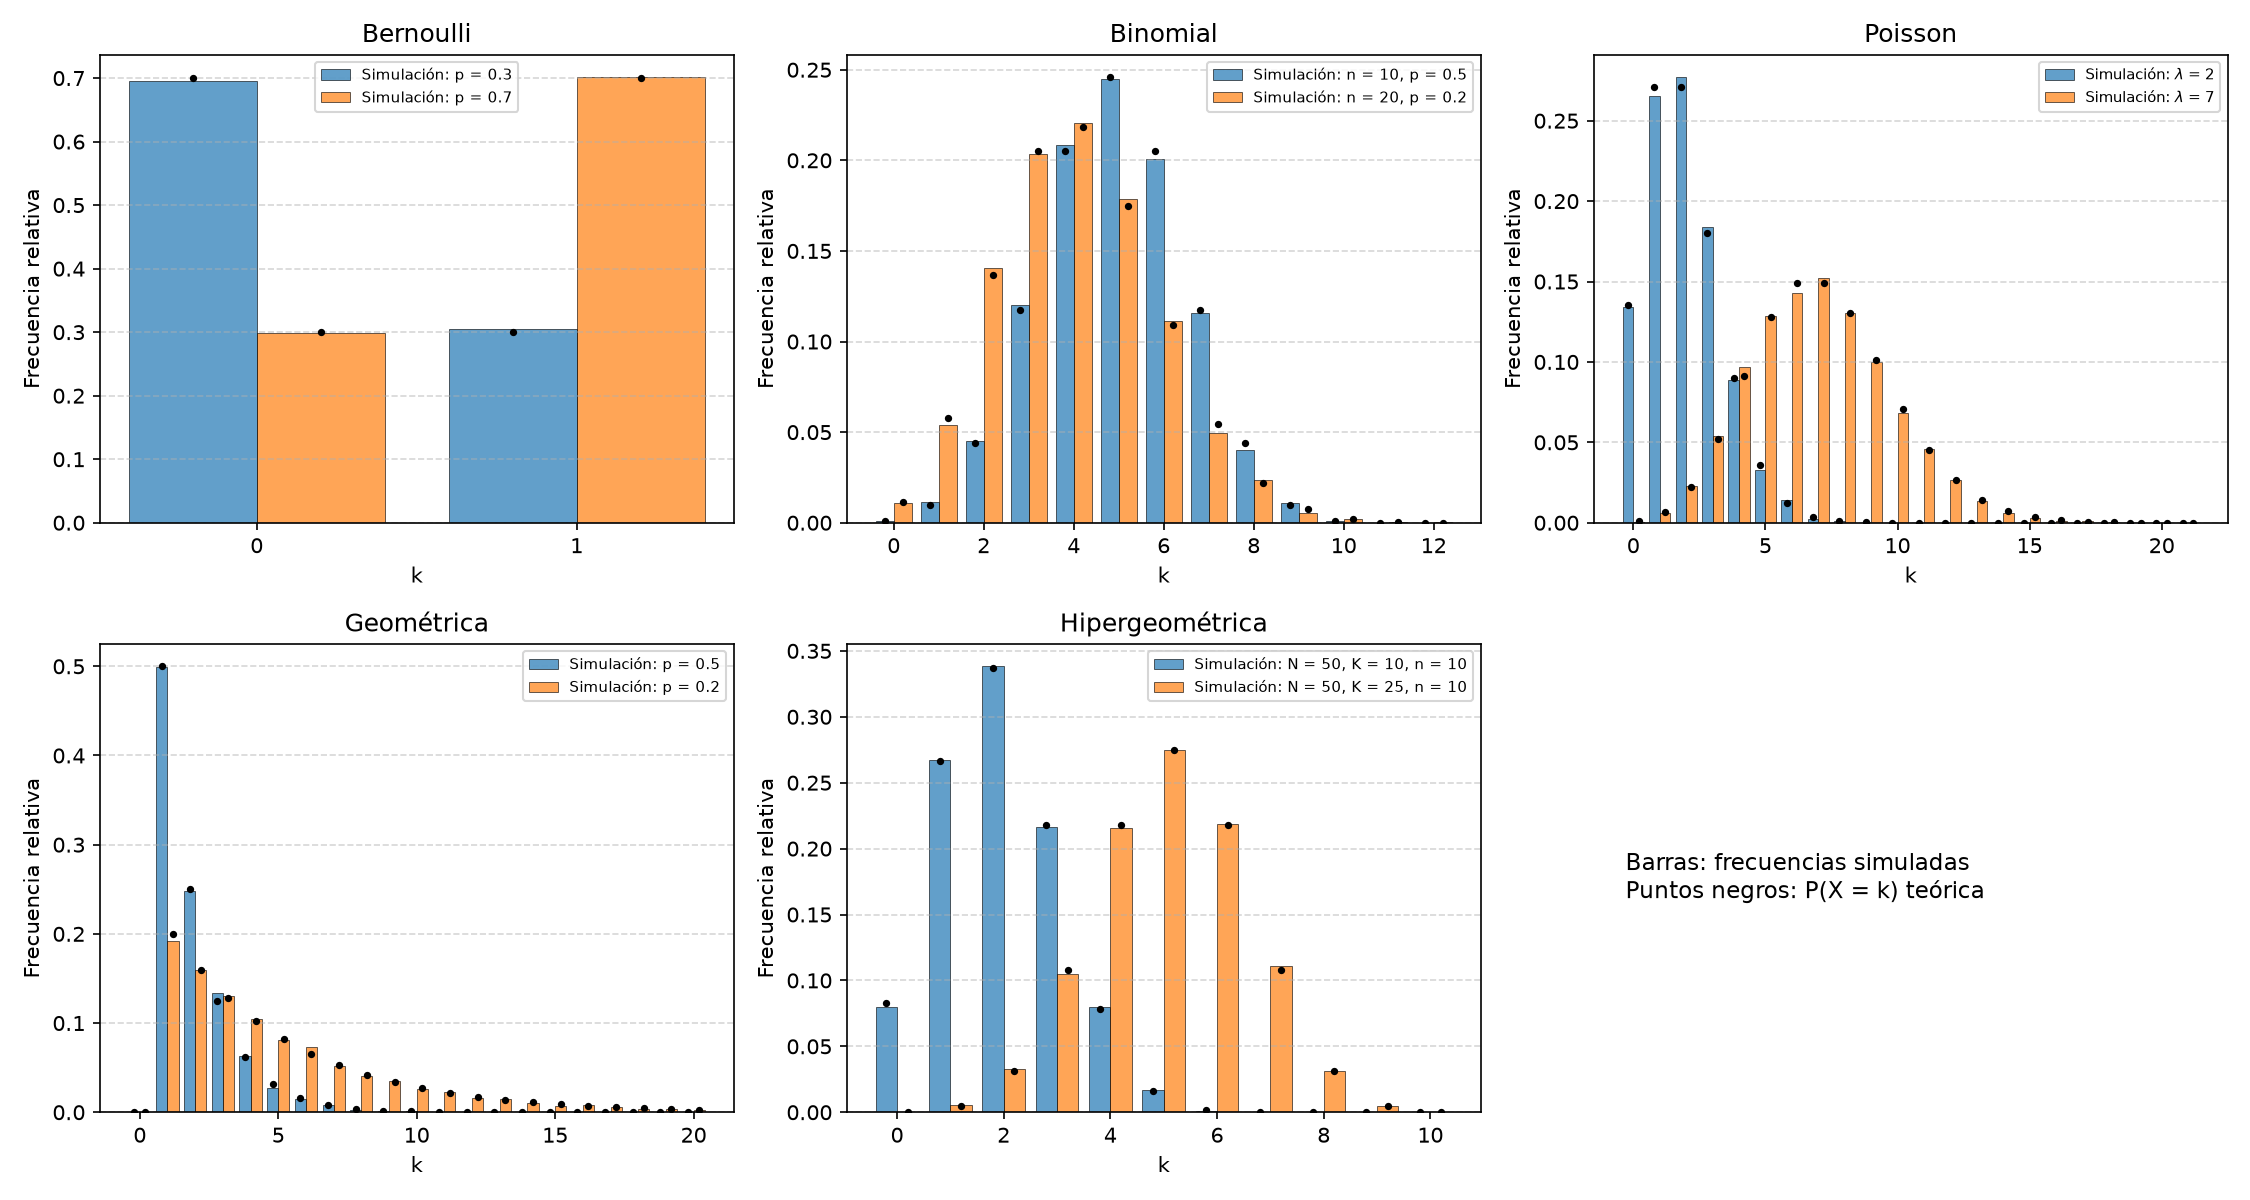
\includegraphics[width=\textwidth]{img/t2_comparacion_distribuciones.png}
\caption{Frecuencias relativas de 10\,000 valores simulados (barras) y $P(X = k)$ teórica (puntos negros) para las cinco distribuciones, con dos conjuntos de parámetros cada una.}
\label{fig:comparacion}
\end{figure}

\begin{figure}[htbp]
\centering
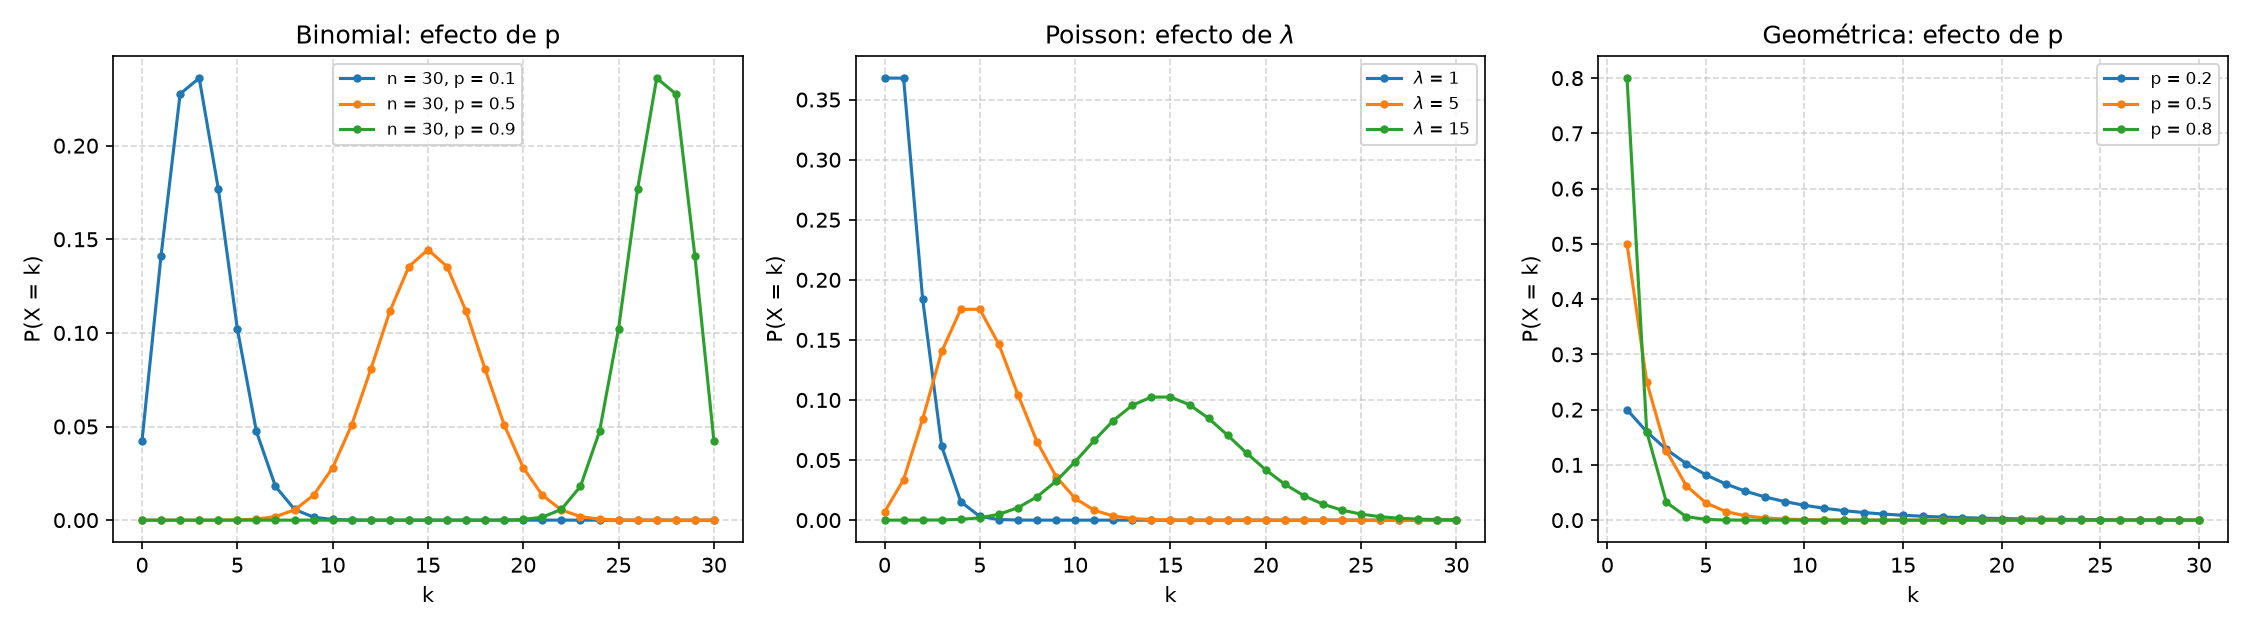
\includegraphics[width=\textwidth]{img/t2_efecto_parametros.png}
\caption{Probabilidades teóricas al variar un parámetro: $p$ en la binomial, $\lambda$ en la Poisson y $p$ en la geométrica.}
\label{fig:parametros}
\end{figure}

\begin{itemize}
    \item \textbf{Bernoulli.} Hay solo dos barras, y su altura es $1 - p$ y $p$. Al pasar de $p = 0.3$ a $p = 0.7$ las barras se intercambian.
    \item \textbf{Binomial.} Con $n = 10$ y $p = 0.5$ la forma es simétrica y centrada en 5; con $n = 20$ y $p = 0.2$ está centrada en 4 y tiene una cola más larga a la derecha.
    \item \textbf{Poisson.} Con $\lambda = 2$ la distribución es asimétrica y se concentra en 0 a 4; con $\lambda = 7$ es más ancha, más baja y casi simétrica.
    \item \textbf{Geométrica.} Siempre es decreciente, con el máximo en $k = 1$ (igual a $p$). Con $p = 0.5$ cae rápidamente; con $p = 0.2$ la cola es larga.
    \item \textbf{Hipergeométrica.} Con 10 bolas negras de 50 el centro está en 2; con 25 de 50 la distribución es simétrica y centrada en 5. Solo toma valores de 0 a $n = 10$.
\end{itemize}

\subsection{Tarea 3: Comparación teórica-empírica}

\begin{consola}[label=out:t3a]{Ejecución de \texttt{act10.py}: media y varianza}
=== Tarea 3a: media y varianza, teóricas vs simuladas ===
   Distribución             Parámetros  Media teórica  Media simulada  Var. teórica  Var. simulada
      Bernoulli                p = 0.3            0.3           0.305         0.210          0.212
      Bernoulli                p = 0.7            0.7           0.702         0.210          0.209
       Binomial        n = 10, p = 0.5            5.0           4.966         2.500          2.527
       Binomial        n = 20, p = 0.2            4.0           3.994         3.200          3.103
        Poisson             lambda = 2            2.0           2.000         2.000          1.953
        Poisson             lambda = 7            7.0           6.964         7.000          6.949
     Geométrica                p = 0.5            2.0           1.987         2.000          1.942
     Geométrica                p = 0.2            5.0           5.026        20.000         19.745
Hipergeométrica N = 50, K = 10, n = 10            2.0           2.004         1.306          1.297
Hipergeométrica N = 50, K = 25, n = 10            5.0           5.009         2.041          2.056
\end{consola}
\begin{consola}[label=out:t3b]{Ejecución de \texttt{act10.py}: probabilidades puntuales}
=== Tarea 3b: P(X = k) con la fórmula, y frecuencia simulada ===
   Distribución             Parámetros  k  P teórica  Frec. simulada  Diferencia  Error estándar
      Bernoulli                p = 0.3  1     0.3000          0.3049      0.0049          0.0046
       Binomial        n = 10, p = 0.5  5     0.2461          0.2451     -0.0010          0.0043
       Binomial        n = 20, p = 0.2  4     0.2182          0.2205      0.0023          0.0041
        Poisson             lambda = 2  2     0.2707          0.2773      0.0066          0.0044
        Poisson             lambda = 7  7     0.1490          0.1522      0.0032          0.0036
     Geométrica                p = 0.5  2     0.2500          0.2484     -0.0016          0.0043
     Geométrica                p = 0.2  5     0.0819          0.0807     -0.0012          0.0027
Hipergeométrica N = 50, K = 10, n = 10  1     0.2662          0.2671      0.0009          0.0044
Hipergeométrica N = 50, K = 25, n = 10  5     0.2748          0.2749      0.0001          0.0045
\end{consola}

Las medias y las varianzas simuladas coinciden con las teóricas con diferencias pequeñas (por ejemplo, la varianza de la geométrica con $p = 0.2$ es 20 y la simulada es 19.745). Las diferencias entre la frecuencia simulada y $P(X = k)$ no pasan de 0.0066, es decir, a lo más 1.5 errores estándar. Para la hipergeométrica con $N = 50$, $K = 10$ y $n = 10$, la varianza teórica es 1.306, menor que la de una binomial con $n = 10$ y $p = 0.2$, que sería 1.6: la razón es el factor $(N - n)/(N - 1) = 40/49$, que refleja el muestreo sin reemplazo.

\begin{consola}[label=out:t3c]{Ejecución de \texttt{act10.py}: prueba chi-cuadrada}
=== Tarea 3c: prueba chi-cuadrada de bondad de ajuste ===
   Distribución             Parámetros  Categorías    chi2  p-valor
      Bernoulli                p = 0.3           2  1.1433   0.2849
      Bernoulli                p = 0.7           2  0.1905   0.6625
       Binomial        n = 10, p = 0.5          11  9.5837   0.4777
       Binomial        n = 20, p = 0.2          12 16.8297   0.1130
        Poisson             lambda = 2           9 14.4317   0.0712
        Poisson             lambda = 7          18 17.4572   0.4238
     Geométrica                p = 0.5          11 23.0416   0.0106
     Geométrica                p = 0.2          30 39.6733   0.0894
Hipergeométrica N = 50, K = 10, n = 10           7  2.9763   0.8118
Hipergeométrica N = 50, K = 25, n = 10           9  3.2906   0.9148
\end{consola}

En 9 de las 10 simulaciones la prueba chi-cuadrada no rechaza la distribución teórica al nivel de 0.05. La excepción es la geométrica con $p = 0.5$ ($p$-valor de 0.0106). Con 10 pruebas a ese nivel se espera rechazar alrededor de 0.5 veces por puro azar, y la media, la varianza y las probabilidades puntuales de esa misma simulación coinciden con la teoría, así que este resultado se interpreta como una fluctuación de la muestra y no como un error del simulador. Aun así, es una advertencia útil: una sola prueba no basta para afirmar que un simulador es correcto, por lo que se complementó con las demás comparaciones.

\begin{consola}[label=out:t3d]{Ejecución de \texttt{act10.py}: lotería de California}
=== Tarea 3d: lotería de California (hipergeométrica N = 53, K = 6, n = 6) ===
 k  P teórica  Frec. (200000 sorteos)
 0   0.467716                0.467435
 1   0.400899                0.402105
 2   0.116540                0.115750
 3   0.014126                0.014075
 4   0.000706                0.000630
 5   0.000012                0.000005
 6   0.000000                0.000000
\end{consola}

Las probabilidades teóricas de la hipergeométrica con $N = 53$, $K = 6$ y $n = 6$ (0.4677, 0.4009, 0.1165, 0.0141, $7.06 \times 10^{-4}$, $1.22 \times 10^{-5}$ y $4.36 \times 10^{-8}$) reproducen la tabla del documento fuente. La simulación con 200\,000 sorteos coincide en los primeros valores (0.4674, 0.4021, 0.1158 y 0.0141); para $k \ge 4$ las probabilidades son tan pequeñas que casi no aparecen en la simulación, y para $k = 6$ (una probabilidad de uno entre 22.9 millones) no se observó ningún caso.

\begin{consola}[label=out:t3e]{Ejecución de \texttt{act10.py}: error según el número de simulaciones}
=== Tarea 3e: error máximo según el número de simulaciones ===
        Binomial  Poisson  Geométrica
N
100       0.0449   0.0996      0.0350
300       0.0251   0.0407      0.0200
1000      0.0311   0.0237      0.0240
3000      0.0189   0.0100      0.0100
10000     0.0030   0.0073      0.0058
30000     0.0024   0.0042      0.0023
100000    0.0020   0.0022      0.0026
300000    0.0011   0.0009      0.0006
\end{consola}

\begin{figure}[htbp]
\centering
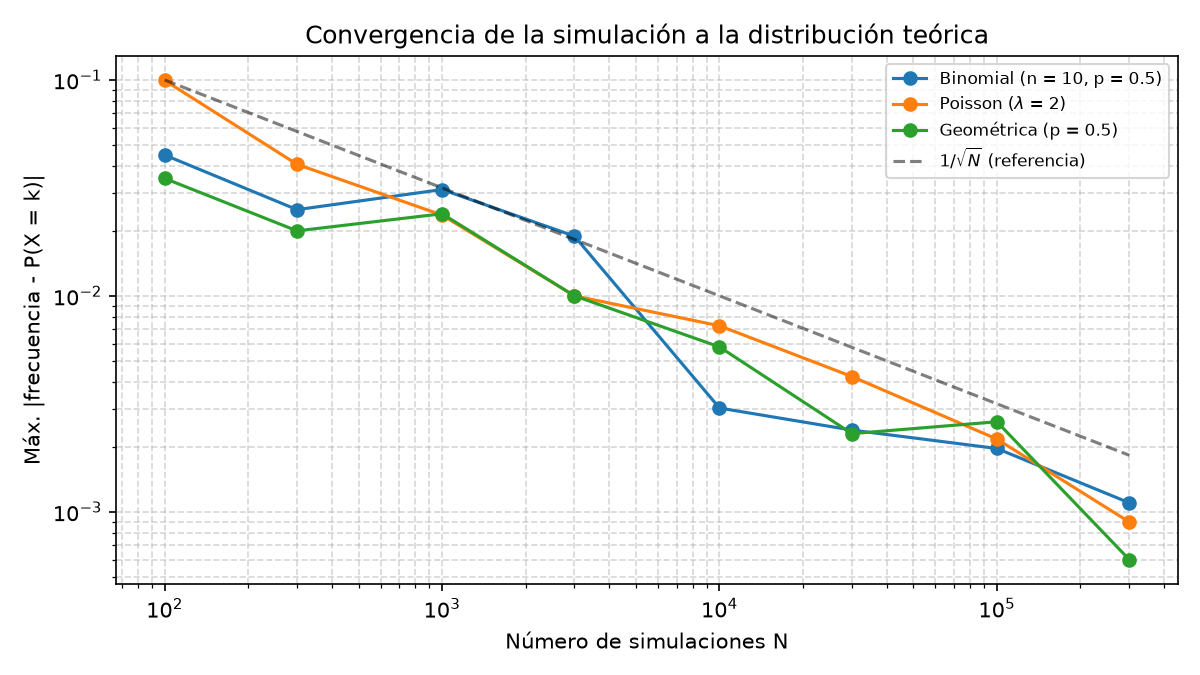
\includegraphics[width=0.8\textwidth]{img/t3_convergencia.png}
\caption{Error máximo entre la frecuencia simulada y $P(X = k)$ según el número de simulaciones (escala logarítmica), con la referencia $1/\sqrt{N}$.}
\label{fig:convergencia}
\end{figure}

El error máximo baja de 0.03 a 0.10 con 100 simulaciones a 0.0006 a 0.0011 con 300\,000, y en la Figura~\ref{fig:convergencia} sigue aproximadamente la pendiente de $1/\sqrt{N}$: para reducir el error diez veces hay que simular unas cien veces más valores. La curva no es suave porque el error máximo es en sí una cantidad aleatoria.

\subsection{Tarea 4: Reflexión final}

La Tabla~\ref{tab:aplicaciones} resume en qué fenómenos se aplica cada distribución y qué efecto tienen sus parámetros, a partir de lo observado en las Figuras~\ref{fig:comparacion} y \ref{fig:parametros}.

\begin{table}[htbp]
\centering
\caption{Aplicaciones y efecto de los parámetros.}
\label{tab:aplicaciones}
\footnotesize
\renewcommand{\arraystretch}{1.3}
\begin{tabular}{p{2.4cm}p{4.8cm}p{6.2cm}}
\hline
\textbf{Distribución} & \textbf{Fenómenos donde se aplica} & \textbf{Efecto de los parámetros en la forma} \\
\hline
Bernoulli & Un solo resultado de sí o no: una moneda, si una pieza sale defectuosa, si un cliente compra \parencite{tecnm2026_documento_fuente}. & $p$ reparte la probabilidad entre 0 y 1; con $p = 0.5$ las barras son iguales y la varianza es máxima. \\
Binomial & Número de éxitos en $n$ ensayos: caras en 10 lanzamientos, piezas defectuosas en un lote inspeccionado con reemplazo. & $p$ desplaza el centro ($np$) y controla la asimetría: simétrica en $p = 0.5$, con cola a la derecha si $p < 0.5$ y a la izquierda si $p > 0.5$. $n$ alarga el rango y la hace más parecida a una campana. \\
Poisson & Conteo de eventos raros e independientes en un intervalo: llamadas a una central, accidentes en una carretera por día, errores tipográficos en una página \parencite{tecnm2026_documento_fuente}. & $\lambda$ fija a la vez el centro y la dispersión (media y varianza son $\lambda$). Con $\lambda$ pequeña es asimétrica con el máximo en 0 o 1; al crecer, se ensancha y se vuelve simétrica. \\
Geométrica & Intentos hasta el primer éxito: boletos de lotería hasta el primer ganador \parencite{tecnm2026_documento_fuente}, intentos de conexión hasta que uno funciona. & $p$ grande concentra la masa en $k = 1$ y la hace caer rápido; $p$ pequeña da una cola larga y una media $1/p$ grande. Siempre es decreciente. \\
Hipergeométrica & Muestreo sin reemplazo de una población finita: aciertos en una lotería, bolas negras extraídas de una urna \parencite{tecnm2026_documento_fuente}, defectuosos en un lote que se inspecciona sin devolver las piezas. & La proporción $K/N$ desplaza el centro ($nK/N$). Su varianza es menor que la de la binomial por el factor $(N - n)/(N - 1)$, y si $N$ es muy grande respecto a $n$ se parece a la binomial. \\
\hline
\end{tabular}
\end{table}

\section{Conclusiones}

Las cinco distribuciones discretas se simularon con dos conjuntos de parámetros, y en todos los casos las medias, las varianzas y las frecuencias simuladas coincidieron con las calculadas con las fórmulas. Las diferencias entre lo empírico y lo teórico fueron del tamaño que predice el error estándar de una proporción, y disminuyeron aproximadamente como $1/\sqrt{N}$ al aumentar el número de simulaciones, de modo que un resultado simulado se acerca a la teoría pero nunca la iguala exactamente. La prueba chi-cuadrada rechazó una de las diez simulaciones, algo compatible con el azar al hacer varias pruebas, lo cual muestra que conviene usar varias comparaciones en lugar de una sola.

Cada distribución corresponde a un patrón de conteo distinto: la Bernoulli a un ensayo, la binomial a los éxitos en $n$ ensayos, la Poisson a eventos raros por intervalo, la geométrica a la espera del primer éxito y la hipergeométrica al muestreo sin reemplazo. Los parámetros controlan el centro, la dispersión y la simetría: $p$ en la binomial y la geométrica, $\lambda$ en la Poisson, que determina a la vez el centro y la dispersión, y $K/N$ en la hipergeométrica. Además se comprobó la relación entre ellas: la hipergeométrica tiene menos varianza que la binomial equivalente por no reemplazar, y la Poisson es el límite de la binomial, como se vio en el documento fuente. Reconocer cuál patrón describe un fenómeno es el primer paso para elegir un modelo de probabilidad en problemas de aprendizaje automático.

\referencias

\end{document}
